% AUTO-GENERATED by scripts/make_tex.py from results/*.csv -- do not edit by hand.

\section{Simulation Setup}

\begin{table}[!t]\centering\caption{Simulation parameters}\label{tab:params}

\begin{tabular}{ll}\hline

Elements = beams $N$ & 16 \\

Replication (paper Sec.~VI) & $f_{\max}=1$~GHz, $\tau=1/(Nf_{\max})=62.5$~ps \\

Course band & 5--10~GHz, $f_{\max}=10$~GHz, $\tau=6.25$~ps \\

Element spacing $d$ & $\lambda_{\min}/2$ (14.99~mm at 10~GHz) \\

Frequency sweep & $f/f_{\max}\in[0.1,1]$, 46 points \\

Angle grid & 4001 points uniform in $\sin\theta\in[-1,1]$ \\

ADVM-b orders & $b\in\{2,3,4,5,6,8\}$ \\

Pass thresholds & squint $<0.5^\circ$, pointing $<0.5^\circ$, SLL loss $<1$~dB \\

\hline\end{tabular}\end{table}

All simulations are frequency-domain array-factor computations with ideal components. Because $d$ and $\tau$ both scale with $1/f_{\max}$, the array factor depends on frequency only through $f/f_{\max}$; the 150~MHz--1~GHz replication and the 5--10~GHz course band are therefore the same simulation read on different frequency axes.

\emph{Sign convention.} A plane wave from $\theta$ reaches element $l$ earlier by $ld\sin\theta/c$, so $x_l=e^{+j2\pi f l d\sin\theta/c}$, and $\alpha=e^{-j\omega\tau}$. A per-element pre-delay $\mathrm{diag}(\alpha^{-Nl/2})$ (anti-causal, absorbed into a common latency) centres the beams so that beam $k'=k-N/2$ of $\tilde{A}_N$ points at $\sin\theta=2k'/N$ at every frequency. The phase-shifter baseline (PS) uses the fixed weights $e^{-j2\pi k'l/N}$ (the DVM at $f_{\max}$) and therefore points at $\sin\theta=(2k'/N)(f_{\max}/f)$.

\emph{Normalization.} Fast algorithms compute $M\hat{A}_N z$ with unnormalized transforms; we divide by $M=2N$ (a bit shift). Pattern plots normalize each beam to 0~dB. Spectral errors are $\min_s\lVert\tilde{A}_N-s\hat{A}_N\rVert_2/\lVert\tilde{A}_N\rVert_2$ over complex $s$. Beam statistics use the beams $|k'|\le N/2-2$ (endfire beams excluded) and, unless stated, the course band $f/f_{\max}\in[0.5,1]$.

\section{Results}

\subsection{Squint}

\begin{figure}[!t]\centering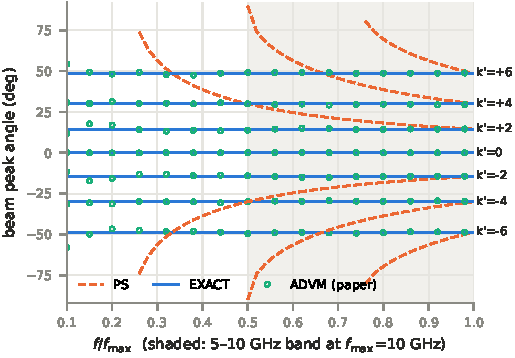
\includegraphics[width=\columnwidth]{../results/figs/F1_peak_vs_freq.pdf}\caption{Beam peak angle versus normalized frequency for $k'\in\{-6,\dots,6\}$. PS (dashed) squints and leaves visible space at low frequency; the TTD (EXACT) beams are flat; ADVM markers stay near EXACT in the band but drift at low frequency.}\label{fig:f1}\end{figure}

Over the course band the squint spread is 60.0$^\circ$ for PS, 1.0e-12$^\circ$ for EXACT and 1.69$^\circ$ for the paper's ADVM (Fig.~\ref{fig:f1}, Table~\ref{tab:methods}). EXACT is squint-free to numerical precision; ADVM exceeds the 0.5$^\circ$ squint-free threshold. Worst-case pointing errors are 60.0$^\circ$ (PS), 6.9e-13$^\circ$ (EXACT) and 1.12$^\circ$ (ADVM). Over the full sweep $f/f_{\max}\in[0.1,1]$ the ADVM pointing error grows to 9.45$^\circ$.

\begin{figure}[!t]\centering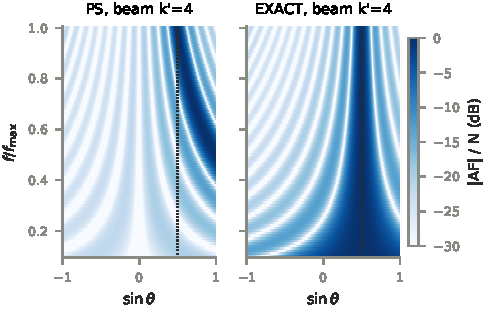
\includegraphics[width=\columnwidth]{../results/figs/F3_heatmap_PS_vs_EXACT.pdf}\caption{$|AF|$ of beam $k'=4$ over $\sin\theta$ and $f/f_{\max}$. PS: tilted ridge (squint). EXACT: vertical ridge at the target (dotted).}\label{fig:f3}\end{figure}

\subsection{Replication of paper Fig.~3}

\begin{figure}[!t]\centering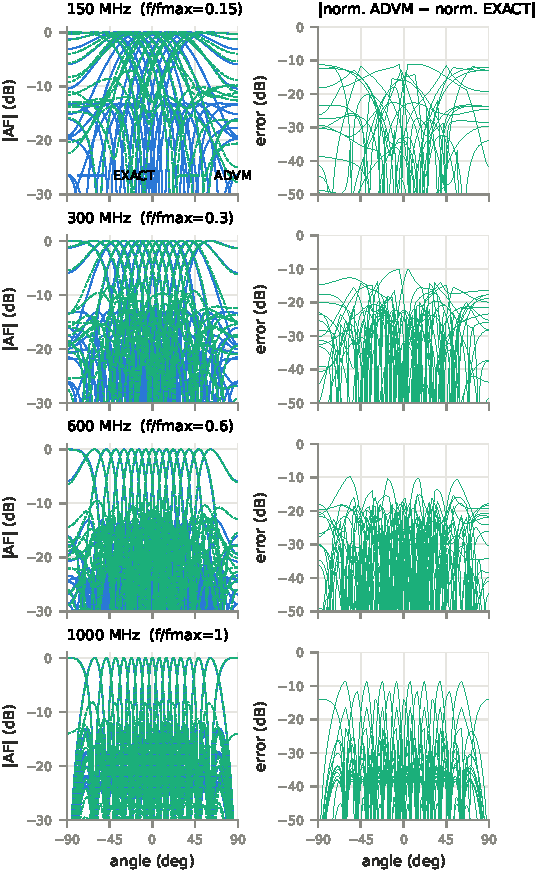
\includegraphics[width=\columnwidth]{../results/figs/F2_paper_fig3_replication.pdf}\caption{All 16 beams at 150, 300, 600 and 1000~MHz ($f_{\max}=1$~GHz). Left: EXACT (solid) vs ADVM (dashed), each beam normalized to 0~dB. Right: magnitude of the difference of the normalized patterns.}\label{fig:f2}\end{figure}

Fig.~\ref{fig:f2} reproduces the paper\textquotesingle s Fig.~3 setup. The ADVM main lobes track EXACT, while the error concentrates in the sidelobe region. The largest normalized-pattern error is -11.1~dB, -10.0~dB, -9.6~dB, -8.5~dB at 150, 300, 600 and 1000~MHz, respectively, and the worst SLL degradation relative to EXACT is 6.8~dB, 5.4~dB, 4.2~dB, 5.0~dB.

\subsection{Complexity}

\begin{figure}[!t]\centering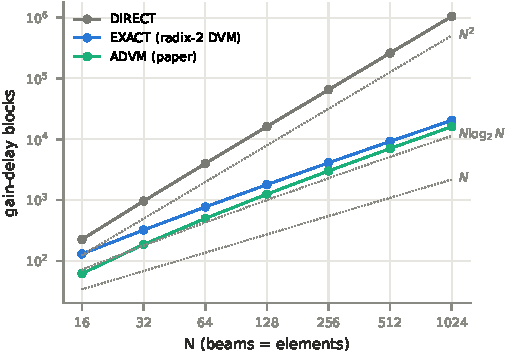
\includegraphics[width=\columnwidth]{../results/figs/F5_complexity.pdf}\caption{Gain-delay blocks counted on the implemented factorizations, with $N^2$, $N\log_2N$ and $N$ reference slopes.}\label{fig:f5}\end{figure}

\begin{table}[!t]\centering\caption{Gain-delay blocks (instrumented) vs.\ paper; area/power reduction (\emph{estimate, proportional model}: area and power $\propto$ gain-delay count)}\label{tab:cx}

\setlength{\tabcolsep}{3pt}\begin{tabular}{rrrrrrr}\hline

$N$ & DIRECT & EXACT & ADVM & Lemma~3.2 & vs DIR. & vs EXACT \\ \hline

16 & 225 & 130 & 62 & 62 & 72.4\% & 52.3\% \\

32 & 961 & 322 & 186 & 186 & 80.6\% & 42.2\% \\

64 & 3969 & 770 & 498 & 498 & 87.5\% & 35.3\% \\

128 & 16129 & 1794 & 1250 & 1250 & 92.2\% & 30.3\% \\

256 & 65025 & 4098 & 3010 & 3010 & 95.4\% & 26.5\% \\

512 & 261121 & 9218 & 7042 & 7042 & 97.3\% & 23.6\% \\

1024 & 1046529 & 20482 & 16130 & 16130 & 98.5\% & 21.2\% \\

\hline\end{tabular}\end{table}

Counting non-trivial multiplications directly on the sparse factors that the code executes reproduces the paper\textquotesingle s Lemma~3.2 for ADVM, its Table~1 counts for the radix-2 DVM, and $(N-1)^2$ for DIRECT at every $N$ (Table~\ref{tab:cx}). At $N=16$ the ADVM needs 62 gain-delay blocks (0 gains, 30 delays, 32 pre-computed anti-causal terms), a 52.3\% reduction versus EXACT and 72.4\% versus DIRECT; at $N=1024$ the reductions are 21.2\% and 98.5\%. The price is adders: at $N=16$ ADVM uses 414 complex additions versus 320 for EXACT. The symmetric-steering pre-delays add $N-1$ delays to every DVM method (not included above).

\subsection{Scalability of the 16-beam building block}

\begin{table}[!t]\centering\caption{ADVM vs EXACT for $N=16,32,64$ (recursion on $\hat{F}_{32}$)}\label{tab:scale}

\setlength{\tabcolsep}{3pt}\begin{tabular}{rrrrrr}\hline

$N$ & $f/f_{\max}$ & patt.\ err (dB) & point.\ err ($^\circ$) & $\Delta$SLL (dB) & rel.\ spec.\ err \\ \hline

16 & 0.15 & -11.1 & 5.27 & 6.8 & 0.300 \\

16 & 0.3 & -10.0 & 1.50 & 5.4 & 0.369 \\

16 & 0.6 & -9.6 & 0.55 & 4.2 & 0.472 \\

16 & 1 & -8.5 & 0.18 & 5.0 & 0.420 \\

32 & 0.15 & -10.1 & 3.58 & 6.5 & 0.328 \\

32 & 0.3 & -11.1 & 0.75 & 4.8 & 0.392 \\

32 & 0.6 & -11.0 & 0.38 & 3.3 & 0.520 \\

32 & 1 & -8.3 & 0.17 & 5.0 & 0.707 \\

64 & 0.15 & -11.3 & 2.76 & 6.4 & 0.316 \\

64 & 0.3 & -12.6 & 0.54 & 5.3 & 0.457 \\

64 & 0.6 & -11.8 & 0.29 & 3.5 & 0.548 \\

64 & 1 & -10.2 & 0.06 & 3.1 & 0.632 \\

\hline\end{tabular}\end{table}

Table~\ref{tab:scale} applies the same ADFT building block recursively for $N=32$ and $64$. The pointing error at a given $f/f_{\max}$ does not grow with $N$, but the relative spectral-norm error stays of order $10^{-1}$ (for $N=16$ it ranges from 0.25 to 0.69 over the sweep).

\subsection{Approximation order (ADVM-b, our extension)}

\begin{figure}[!t]\centering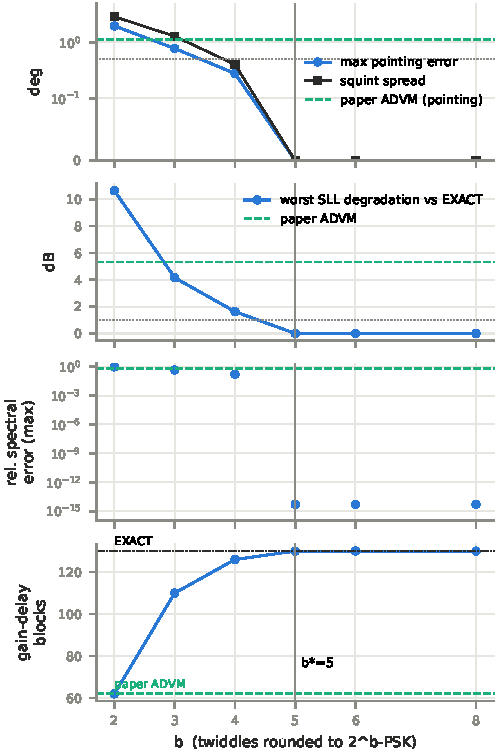
\includegraphics[width=\columnwidth]{../results/figs/F4_bsweep.pdf}\caption{ADVM-b (our extension): twiddles rounded to $2^b$-PSK. Dashed: paper ADVM. Dotted: pass thresholds. Bottom: gain-delay blocks at $N=16$.}\label{fig:f4}\end{figure}

As a separate experiment that is \emph{not} part of the paper, we rounded every twiddle of the exact radix-2 transform to the nearest $2^b$-PSK phase (Fig.~\ref{fig:f4}). The smallest order meeting all three criteria is $b^*=5$. This result is trivial rather than a trade-off: for $N=16$ every twiddle of the 32-point DFT already lies on the 32-PSK grid, so $b\ge5$ is EXACT and costs as much (130 blocks). The informative point is $b=4$ (126 blocks): squint spread 0.40$^\circ$ and pointing error 0.28$^\circ$ pass, but the SLL loss of 1.63~dB fails the 1~dB limit. At the paper\textquotesingle s gain-delay budget (62, i.e.\ $b=2$), rounding is worse than the paper\textquotesingle s ADFT (SLL loss 10.6~dB vs 5.3~dB).

\subsection{Summary of methods}

\begin{figure}[!t]\centering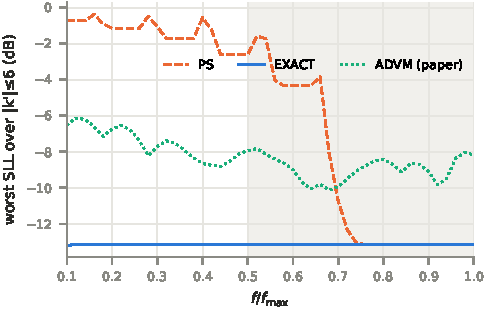
\includegraphics[width=\columnwidth]{../results/figs/F6_sll_vs_freq.pdf}\caption{Worst sidelobe level over beams $|k'|\le6$ versus frequency.}\label{fig:f6}\end{figure}

\begin{table}[!t]\centering\caption{Methods $\times$ metrics, $N=16$, course band (worst case over $|k'|\le6$)}\label{tab:methods}

\setlength{\tabcolsep}{2pt}\begin{tabular}{lrrrrrrc}\hline

Method & squint & point. & gain var. & SLL & $\Delta$SLL & GD & pass \\

 & ($^\circ$) & ($^\circ$) & (dB) & (dB) & (dB) & blocks & \\ \hline

PS & 60.00 & 60.00 & 17.49 & -1.59 & 11.56 & n/a & no \\

EXACT & 0.00 & 0.00 & 0.00 & -13.15 & 0.00 & 130 & yes \\

ADVM & 1.69 & 1.12 & 3.51 & -7.82 & 5.32 & 62 & no \\

ADVM-b (b=2) & 2.89 & 1.97 & 4.28 & -2.51 & 10.64 & 62 & no \\

ADVM-b (b=3) & 1.29 & 0.78 & 1.63 & -8.99 & 4.16 & 110 & no \\

ADVM-b (b=4) & 0.40 & 0.28 & 0.39 & -11.52 & 1.63 & 126 & no \\

ADVM-b (b=5) & 0.00 & 0.00 & 0.00 & -13.15 & 0.00 & 130 & yes \\

ADVM-b (b=6) & 0.00 & 0.00 & 0.00 & -13.15 & 0.00 & 130 & yes \\

ADVM-b (b=8) & 0.00 & 0.00 & 0.00 & -13.15 & 0.00 & 130 & yes \\

\hline\end{tabular}\end{table}

\section{Discussion and Limitations}

\begin{enumerate}

\item \emph{The paper\textquotesingle s ADVM does not meet our criteria.} It halves the gain-delay count at $N=16$ but loses up to 5.3~dB of sidelobe level in the course band (7.0~dB over the full sweep), has 3.5~dB peak-gain variation and 1.69$^\circ$ residual squint. The paper reports a 1--2~dB SLL penalty. We could not reconcile this; one possible cause is the dB convention of the paper\textquotesingle s Fig.~4, where the EXACT sidelobes appear well above the -13.1~dB we obtain for a uniform 16-element array. We did not verify this. The thresholds were fixed before running and were not changed.

\item Multiplication by $\pm j$ is treated as free. In hardware this assumes an ideal wideband $90^\circ$ element (hybrid coupler or Hilbert transformer), which itself has finite bandwidth and error.

\item All delays are ideal: no waveguide or transmission-line dispersion, loss, mismatch, or quantization of the delay values, and the antenna elements are isotropic with no mutual coupling. The results are array-factor computations, not full-wave or measured data.

\item Area and power figures are an \emph{estimate from a proportional model} (area, power $\propto$ gain-delay count, following the paper). Adders, routing and the anti-causal latency are not costed; ADVM needs more adders than EXACT.

\item ADVM-b is our own extension and is not from the paper. For $N=16$ it only reproduces EXACT once $b\ge5$, so it offers no cheaper squint-free design point at this size.

\item The paper\textquotesingle s Fig.~3/4 beams lie on one side of broadside and its element spacing is not stated. We steer symmetrically about broadside, so the replication matches the paper\textquotesingle s set-up and trends, not its exact beam angles.

\end{enumerate}
